\section{Tutorial - Fast Fourier Transformation }

\subsection{Introduction}

\begin{frame}
\frametitle{Fast Fourier Transformation}

Speeds up calculations of DFT (Discrete Fourier transform)

Used for fast:
\begin{itemize}
\item Addition of polynomials
\item Multiplication of polynomials
\item Conversion between Coefficient Representation \& Point-value Representation
\end{itemize}
% Interpolate - Evaluate

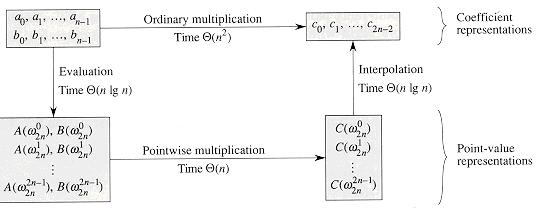
\includegraphics[scale=0.5]{images/poly-transform.jpg}

\end{frame}

\subsection{Polynomials}

\begin{frame}
\frametitle{Polynomials}
\begin{equation}
A(x) = \sum{^{n-1}_{j=0} \hspace{0.5em} a_jx^i}, \hspace{1.5em} a_j x^3 + a_{j-1} x^2 - a_{j-2} x + 4
\end{equation}


\textbf{Degree:} highest non-zero coefficient 

\textbf{Degree-bound:} Any integer strictly larger than the bound for $A(x)$

\end{frame}


\begin{frame}
\frametitle{Polynomial Addition}

\begin{eqnarray}
A(x) = 6x^3 + 7x^2 - 10x + 9  \\
B(x) = -2x^3 + 4x -5  \\ \hline
C(x) = 4x^3 + 7x^2 - 6x + 4 
\end{eqnarray}


\begin{eqnarray*}
\begin{tabular}{ l r }
 A(x) = & 6x^3 + 7x^2 - 10x + 9  \\
 B(x) = & -2x^3 + 4x -5  \\ \hline
 C(x) = & 4x^3 + 7x^2 - 6x + 4 
 \end{tabular}
\end{eqnarray*}


\end{frame}


\begin{frame}
\frametitle{Polynomial Multiplication}

\begin{itemize}
\item 
\end{itemize}


\end{frame}

\begin{frame}
\frametitle{Fast Fourier Transformation}


\begin{itemize}
\item 
\end{itemize}
% Interpolate - Evaluate



\end{frame}

